\documentclass[12pt,a4paper]{article}

\usepackage[T5]{fontenc}
\usepackage[utf8]{inputenc}
\usepackage[a4paper,margin=2.5cm]{geometry}
\usepackage{amsmath,amssymb}
\usepackage{graphicx,float,caption,booktabs,array,xcolor,listings,fancyhdr,enumitem}
\usepackage[colorlinks=true,linkcolor=black,urlcolor=blue]{hyperref}
\usepackage{mathtools,amssymb}


\newcommand{\hocky}{HK261}
\newcommand{\mamon}{CO2036}
\newcommand{\ngaynop}{7/11/2026}   
\newcommand{\thanhvien}{%
  \textit{Phạm Huỳnh Trọng Trí} -- \textit{2213657}}

\newcommand{\khunghinh}[3]{
  \begin{figure}[H]
    \centering
    \fbox{\rule{0pt}{#1}\rule{0.85\textwidth}{0pt}}
    \caption{#2}\label{#3}
  \end{figure}}

% ---------- Dinh dang code Scilab ----------
\lstdefinelanguage{Scilab}{
  morekeywords={for,end,if,then,else,elseif,while,function,endfunction,return,clear,clc,isdef},
  sensitive=true, morecomment=[l]{//}, morestring=[b]"}
\lstset{
  language=Scilab, basicstyle=\ttfamily\small, keywordstyle=\color{blue}\bfseries,
  commentstyle=\color{teal}\itshape, stringstyle=\color{orange!70!black},
  numbers=left, numberstyle=\tiny\color{gray}, frame=single, breaklines=true,
  columns=fullflexible, showstringspaces=false, xleftmargin=1.5em, framexleftmargin=1.5em}

% ---------- Header / footer ----------
\pagestyle{fancy}
\fancyhf{}
\lhead{Xử lý tín hiệu số}
\chead{\hocky}
\rhead{\mamon}
\cfoot{\thepage}
\renewcommand{\headrulewidth}{0.4pt}

\newcommand{\Z}{\xleftrightarrow{\;\mathcal{Z}\;}}
\renewcommand{\arraystretch}{1.25}

\begin{document}

% ======================= TRANG BIA =======================
\begin{center}
  {\Large BÀI THỰC HÀNH XỬ LÝ TÍN HIỆU SỐ}\\[1.2em]
  {\Large Lab\ 4 -- Phân tích hệ thống bằng biến đổi Z}\\[1.5em]
  \thanhvien\\[1.5em]
  \ngaynop
\end{center}

\section*{Tổng quan}
Báo cáo này trình bày các bài thực hành của Lab 4 trong học phần Xử lý tín hiệu số, gồm:
tìm biến đổi Z và miền hội tụ (ROC) của tín hiệu rời rạc, khảo sát các thư viện âm thanh và
ảnh số trong Scilab, và tính tích chập tuyến tính, tích chập vòng bằng ba cách: gấp -- dời,
ma trận và kiểm tra bằng hàm có sẵn. Kết quả tính tay được đối chiếu với kết quả mô phỏng.

\section*{Mục tiêu}
\begin{itemize}[nosep]
  \item Xác định biến đổi Z và ROC của tín hiệu hữu hạn, nhân quả và hai phía.
  \item Làm quen các hàm xử lý âm thanh và ảnh số trong Scilab.
  \item Tính tích chập tuyến tính và tích chập vòng bằng phương pháp gấp -- dời và phương pháp ma trận.
  \item Biểu diễn tín hiệu và năng lượng của tín hiệu bằng đồ thị trong Scilab.
\end{itemize}

\section*{Phương pháp}
Các bài biến đổi Z dùng bảng cặp biến đổi cơ bản và tính chất tuyến tính. ROC của tổng là giao
các ROC thành phần. Các bài mô phỏng được viết bằng Scilab và đối chiếu với kết quả tính tay.

\begin{table}[H]
\centering
\begin{tabular}{lcc}
\toprule
Dãy $x(n)$ & $X(z)$ & ROC \\
\midrule
$\delta(n)$ & $1$ & mọi $z$ \\
$\delta(n-m)$ & $z^{-m}$ & mọi $z$ trừ $0$ hoặc $\infty$ \\
$a^n u(n)$ & $\dfrac{1}{1-az^{-1}}$ & $|z|>|a|$ \\
$-a^n u(-n-1)$ & $\dfrac{1}{1-az^{-1}}$ & $|z|<|a|$ \\
$n a^n u(n)$ & $\dfrac{az^{-1}}{(1-az^{-1})^2}$ & $|z|>|a|$ \\
\bottomrule
\end{tabular}
\caption{Các cặp biến đổi Z được sử dụng.}
\end{table}

% ======================= PHAN 1 =======================
\section{Bài tập biến đổi Z (Bài 1--3)}

\subsection{Bài 1}
$x(n)=2\delta(n+2)-\delta(n+1)+2\delta(n)-3\delta(n-1)+4\delta(n-2)$.

Dùng $\delta(n-m)\Z z^{-m}$:
\[
X(z)=2z^{2}-z+2-3z^{-1}+4z^{-2}.
\]
Có số hạng $z^{2}$ nên $z=\infty$ không thuộc ROC. Có số hạng $z^{-2}$ nên $z=0$ không thuộc ROC.

\textbf{ROC:} mọi $z$ trừ $0$ và $\infty$.

\subsection{Bài 2}
$x(n)=0{,}5^n u(n)+0{,}4^n u(n)$.

\begin{align*}
x_1(n)=0{,}5^n u(n)&\Z X_1(z)=\frac{1}{1-0{,}5z^{-1}},\quad |z|>0{,}5,\\
x_2(n)=0{,}4^n u(n)&\Z X_2(z)=\frac{1}{1-0{,}4z^{-1}},\quad |z|>0{,}4.
\end{align*}
Cộng hai thành phần, quy đồng:
\[
X(z)=\frac{(1-0{,}4z^{-1})+(1-0{,}5z^{-1})}{(1-0{,}5z^{-1})(1-0{,}4z^{-1})}
=\frac{2-0{,}9z^{-1}}{1-0{,}9z^{-1}+0{,}2z^{-2}}
=\frac{z(2z-0{,}9)}{(z-0{,}5)(z-0{,}4)}.
\]
ROC là giao của hai ROC thành phần: \textbf{$|z|>0{,}5$}. Hai cực tại $z=0{,}5$ và $z=0{,}4$.

\subsection{Bài 3}
$x(n)=0{,}5^n u(n)+0{,}9^n u(-n-1)$.

Thành phần thứ hai mang dấu ngược so với bảng, vì $-0{,}9^n u(-n-1)\Z \frac{1}{1-0{,}9z^{-1}}$ với $|z|<0{,}9$. Do đó
\[
X(z)=\frac{1}{1-0{,}5z^{-1}}-\frac{1}{1-0{,}9z^{-1}}
=\frac{-0{,}4z^{-1}}{1-1{,}4z^{-1}+0{,}45z^{-2}}
=\frac{-0{,}4z}{(z-0{,}5)(z-0{,}9)}.
\]
ROC là giao của $\{|z|>0{,}5\}$ và $\{|z|<0{,}9\}$, tức \textbf{$0{,}5<|z|<0{,}9$} (hình vành khuyên).

% ======================= PHAN 2 =======================
\section{Bài tập Scilab bổ sung}

\subsection{Bài 4 Xử lý âm thanh}
Scilab cung cấp các hàm cơ bản sau (tên hàm có thể khác nhau tùy phiên bản, cần kiểm tra bằng \texttt{help}):
\begin{itemize}[nosep]
  \item \texttt{audioread}, \texttt{audiowrite} (Scilab 6.x), hoặc \texttt{wavread}, \texttt{wavwrite} (bản cũ): đọc và ghi file WAV.
  \item \texttt{sound}, \texttt{playsnd}: phát tín hiệu âm thanh.
  \item \texttt{plot}, \texttt{fft}: vẽ dạng sóng và phân tích phổ.
\end{itemize}

Ví dụ: tạo tín hiệu sin 440~Hz, ghi ra file, đọc lại, vẽ dạng sóng và phổ biên độ.
\begin{lstlisting}
fs = 8000; t = 0:1/fs:1-1/fs;
x  = 0.5*sin(2*%pi*440*t);   

if isdef("audiowrite") then
    audiowrite("sin440.wav", x, fs);
    [y, fs2] = audioread("sin440.wav");
else
    wavwrite(x, fs, "sin440.wav");
    [y, fs2] = wavread("sin440.wav");
end
y = y(:)';

clf(); subplot(2,1,1);
plot(t(1:40), y(1:40)); xtitle("440 Hz, 5 ms dau", "t (s)", "bien do"); xgrid();

Y = abs(fft(y))/length(y);
f = (0:length(y)-1)*fs/length(y);
subplot(2,1,2);
plot(f(1:length(f)/2), Y(1:length(f)/2));
xtitle("Pho bien do", "f (Hz)", "|Y|"); xgrid();
\end{lstlisting}
Kết quả mong đợi: phổ biên độ có một đỉnh tại $440$~Hz.

\begin{figure}[htbp]
    \centering
    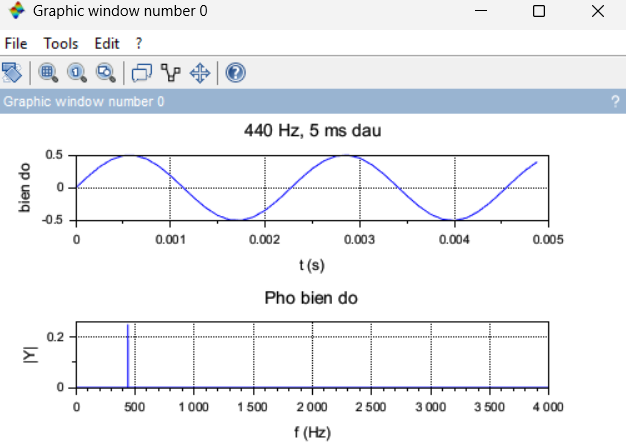
\includegraphics[width=0.7\textwidth]{bai4lab4.png}
    \caption{Dạng sóng và phổ biên độ của tín hiệu sin 440 Hz.}
    \label{fig:audio}
\end{figure}

\subsection{Bài 5 Xử lý ảnh}
Ảnh thử là ảnh xám $64\times64$ có tương phản thấp (giá trị chỉ nằm trong khoảng $80$--$140$), nên tác dụng của cân bằng histogram thể hiện rõ. Chương trình chỉ dùng hàm lõi của Scilab; nếu máy có SIVP hoặc IPCV, có thể thay bằng \texttt{imread}, \texttt{imshow} và các hàm lọc tương ứng.

\begin{lstlisting}
[X, Y] = meshgrid(1:64, 1:64);
I = round(80 + 40*(X/64) + 20*(((X-32).^2 + (Y-32).^2) < 15^2));

// 1) Histogram
h = zeros(1,256);
for v = 0:255, h(v+1) = sum(I == v); end

// 2) Can bang histogram
cdf  = cumsum(h)/sum(h);
cmin = min(cdf(cdf > 0));
Ieq  = round(255*(matrix(cdf(I(:)+1), size(I)) - cmin)/(1 - cmin));

// 3) Lam mo: loc trung binh 3x3
Ib = round(conv2(I, ones(3,3)/9, "same"));

// 4) Watermark: tron alpha
W = zeros(I); W(52:60, 4:60) = 255;
Iw = round(0.8*I + 0.2*W);

f = scf(0); clf(); f.color_map = graycolormap(256);
subplot(2,3,1); Matplot(I+1);   xtitle("Anh goc");
subplot(2,3,2); Matplot(Ieq+1); xtitle("Can bang histogram");
subplot(2,3,3); Matplot(Ib+1);  xtitle("Lam mo 3x3");
subplot(2,3,4); Matplot(Iw+1);  xtitle("Watermark");
subplot(2,3,5); plot2d3(0:255, h);  xtitle("Histogram goc");
he = zeros(1,256); for v=0:255, he(v+1) = sum(Ieq == v); end
subplot(2,3,6); plot2d3(0:255, he); xtitle("Histogram sau can bang");
\end{lstlisting}

\begin{figure}[htbp]
    \centering
    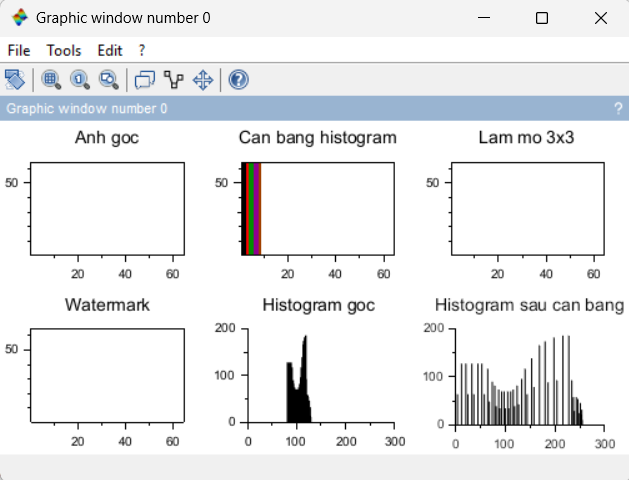
\includegraphics[width=0.7\textwidth]{bai5lab4.png}
    \caption{Ảnh gốc, ảnh sau cân bằng histogram, làm mờ, watermark và các histogram}
    \label{fig:bai5}
\end{figure}


\begin{thebibliography}{9} \url{https://github.com/nhd000/HK261_Report_L02_Lab4_2213657}
\end{thebibliography}
\end{document}

